% LaTeX-Vorlage zur Erstellung einer Abschlussarbeit in der Fakultät Elektrotechnik, Medien und Informatik an der OTH Amberg-Weiden
% Diese Vorlage entstand im Rahmen des Kurses "LaTeX fürs Studium"
% Aktuelle Version: v0.03bacsem
% Stand: 18.04.2020
%
% Changelog:
%
% v0.03bacsem-us: 28.04.2020, Grafikpfad und Bibliographiemanagement 
%                             via bibtex hinzugefügt
% Grafikpfad für das graphicx-Paket:
%   \graphicspath{{images/}} % hinter \usepackage{graphicx}
% Literaturverzeichnis nach DIN:          
%   \usepackage[square,numbers,sort]{natbib} 
% Literaturverzeichnis am Ende:
%   \bibliographystyle{natdin}
%   \bibliography{literatur}
% 
% v0.02: 06.08.2015, Anpassung der Vorlage:
% + Persönliche Informationen (Vorname, Name, Titel usw.) werden direkt in die PDF-Dokumenteinstellungen übernommen
% + Korrektur der Verlinkung von Abbildungs- und Tabellenverzeichnis aus dem Inhaltsverzeichnis (phantomsection) bzw. deren Seitenzahl
%   Besten Dank für diesen Hinweis an Jan-Olaf Becker
% + Anpassung des Namens der Fakultät nach deren Umbenennung
%
% v0.01: 14.03.2012, Erstellung der Vorlage
% oneside: legt Seitennummerierung in die Mitte -> einseitiger Druck
% twoside: legt Seitennummerierung abh. von Seite an rechten/linken Rand -> vorder-/rueckseite Druck
\documentclass[12pt,oneside]{report}
\usepackage[T1]{fontenc}		% Einstellungen fuer Umlaute usw.
\usepackage[utf8x]{inputenc}
\usepackage[ngerman]{babel}

\usepackage{parskip}			% Einstellungen fuer Absaetze: Abstand statt Einrueckung

\usepackage[a4paper,			% Papierformat A4
	    left=2.0cm,				% linker Rand
	    right=2.0cm,			% rechter Rand
	    top=2.0cm,				% oberer Rand
	    bottom=2.0cm,			% unter Rand
	    marginparsep=5mm,		% Abstand der Randnotizen
	    marginparwidth=10mm, 	% Breite der Randnotizen
	    headheight=7mm,			% Hoehe der Kopfzeile
	    headsep=1.2cm,			% Abstand der Kopfzeile
	    footskip=1.5cm,			% Abstand der Fusszeile
	    includeheadfoot]{geometry}

\usepackage{fancyhdr}						% Konfiguration von Kopf- und Fusszeilen
\pagestyle{fancy}							% Seitenstil 'fancy'
\fancyhf{}									% vorhandene Einstellungen loeschen
\setlength{\headwidth}{\textwidth}			% Kopf- und Fusszeile so breit wie der Haupttext
\fancyfoot[R]{\thepage} 					% Festlegung des Seitenstils: Seitenzahlen in der Fusszeile rechts
\fancyfoot[L]{\leftmark}					% Kapitelnr. und -Bezeichnung in der Fusszeile links
\fancyhead[R]{\IhreArbeit}					% "Bachelorarbeit" in der Kopfzeile rechts
\fancyhead[L]{\IhrVorname\ \IhrNachname}	% Vorname und Name in der Kopfzeile links
\renewcommand{\chaptermark}[1]{			% Definition der Ausgabe des Kapitels
  \markboth{Kapitel \thechapter. #1}{}}
\renewcommand{\headrulewidth}{0.5pt}		% Trennlinie zwischen Kopfzeile und Haupttext
\renewcommand{\footrulewidth}{0.5pt}		% Trennlinie zwischen Haupttext und Fusszeile
\fancypagestyle{plain}{					% Anpassung des Seitenstils 'plain' bei Beginn neuer Kapitel
  \fancyhf{}								% Vorbelegung loeschen
  \fancyfoot[C]{\thepage}					% Seitenzeilen in der Fusszeile mittig
  \fancyhead[R]{\IhreArbeit}				% "Bachelorarbeit" in der Kopfzeile rechts
  \fancyhead[L]{\IhrVorname\ \IhrNachname}	% Vorname und Name in der Kopfzeile links
}

%\usepackage{amsmath}			% Pakete fuer den Mathematikmodus
%\usepackage{amssymb}
\usepackage[intlimits]{empheq}

\usepackage[sc]{mathpazo}		% Schriftart Palatino fuer Haupttext und Mathematikmodus
\usepackage{pifont}				% zusaetzliche Symbole

\usepackage{setspace}
\setstretch{1.25}

\usepackage[format=hang,		% Einstellung fuer Bildunterschriften
            font={footnotesize},
            labelfont={bf},
            margin=1cm,
            aboveskip=5pt,
            position=bottom]{caption}

\usepackage{graphicx}	   % Einbinden von Grafiken (jpg, png, pdf, ...)
\graphicspath{{images/}}   % Suchpfad für Grafikdateien

\usepackage[svgnames,table,hyperref]{xcolor} 	% Verwendung von Farben
\usepackage{tikz}								% Erstellen von Grafiken
\usetikzlibrary{positioning,arrows,plotmarks} % TikZ-Bibliotheken
%\usepackage{pgfplots}                           % Darstellung von Plots, Funktionen, Graphen usw.

%
% Weitere Pakete
%
\usepackage{listings}			% Darstellung von Quellcode
\definecolor{mygreen}{rgb}{0,0.6,0}
\definecolor{myblue}{rgb}{0.0,0.0,1.0}
\definecolor{myred}{rgb}{1.0,0.3,0.0}

\DeclareMathOperator{\arctantwo}{arctan2}

\usepackage{leftidx}

\lstset{language = Python,
	numbers = none,
	basicstyle = \small\ttfamily,
	keywordstyle = \color{myblue},
	commentstyle = \color{mygreen},
	stringstyle = \color{myred},
	columns = flexible,
	showstringspaces = false,
	frame = single,
	morekeywords={as, family}
}
\usepackage{float}
\usepackage[square,numbers,sort]{natbib} % Referenzen
%
%\usepackage[european, siunitx]{circuitikz}	% Darstellung von Schaltungen
%
%\usepackage{enumerate}			% Formatierung nummerierter Listen

\usepackage{microtype,relsize}					% Wird verwendet, um Nachnamen auf Titelseite gesperrt darzustellen
\newcommand*{\Sperren}[1]{\textls*[100]{#1}}

% 
% Persoenliche Angaben
% 
\newcommand*{\IhrVorname}{André}
\newcommand*{\IhrNachname}{Kestler}
\newcommand*{\IhrStudiengang}{Künstliche Intelligenz}
% Bachelorarbeit, Masterarbeit, Studienarbeit
\newcommand*{\IhreArbeit}{Studienarbeit Deep Vision}
\newcommand*{\IhrTitelDE}{Vergleich der YOLOX- und YOLOv8-Modelle für die Objekterkennung im Kontext des Udacity Self Driving Car-Datensatzes}
\newcommand*{\IhrBearbeitungszeitraumVON}{21. Juni 2023}
\newcommand*{\IhrBearbeitungszeitraumBIS}{19. Juli 2023}
\newcommand*{\IhrErstpruefer}{Prof. Dr. phil. Tatyana Ivanovska}


\usepackage[bookmarks, raiselinks, pageanchor, % PDF-Einstellungen
            hyperindex, colorlinks,
            citecolor=black, linkcolor=black,
            urlcolor=black, filecolor=black,
            menucolor=black]{hyperref}
\hypersetup{pdftitle={\IhrTitelDE},%
            pdfauthor={\IhrVorname\ \IhrNachname},%
            pdfsubject={\IhreArbeit}}

%
% Beginn des Textteils
%
\begin{document}
    \pagenumbering{roman}
  \thispagestyle{empty}
  \begin{center}
    \Large
    Ostbayerische Technische Hochschule Amberg-Weiden\\
    Fakultät Elektrotechnik, Medien und Informatik\\[1cm]
    Studiengang \IhrStudiengang\\[1cm]
    \textbf{\IhreArbeit}\\[1cm]
    von\\[1cm]
    \IhrVorname\ \Sperren{\textbf{\IhrNachname}}\\[1cm]
    \textbf{\IhrTitelDE}\\[1cm]
%    \IhrTitelE
  \end{center}
  \vspace*{2.5cm}
  \begin{tabbing}
    \underbar{Bearbeitungszeitraum:}\qquad\= von\qquad\=\IhrBearbeitungszeitraumVON\\
                                          \> bis      \>\IhrBearbeitungszeitraumBIS
  \end{tabbing}
  \vspace*{1cm}
  \underbar{1. Prüfer:}\qquad\IhrErstpruefer\par 
 % \underbar{2. Prüfer:}\qquad\IhrZweitpruefer
    \tableofcontents
    \thispagestyle{empty}
 	\newpage
  
% ----------------------------------------------------------------------  
  
%  \chapter*{Symbole, Formelzeichen und Einheiten}
 % \begin{tabular}{ll}
 % 	%$I$ & Einheitsmatrix\\
 % 	%GB     & Gigabyte ($10^9$ Bytes)\\
 % \end{tabular}
 % \newpage
  
% ----------------------------------------------------------------------  
  \chapter*{Abkürzungsverzeichnis}
    \begin{tabular}{ll}
    	%KI	& Künstliche Intelligenz\\
    	%TCP & Tool Center Point\\  		
    	AR & Augmented Reality\\
    	VR & Virtual Reality\\
    	MR & Mixed Reality
  	\end{tabular}

  \newpage
  \pagenumbering{arabic}
  % Kapitel einfügen
  
  \chapter{Einleitung}

\section{Aufgabenstellung}
Im Rahmen der Vorlesung Deep Vision ist ein Projekt im Themenbereich des Kurses zu bearbeiten. Die Bearbeitung erfolgt als Einzelarbeit. Als Projekt werden zwei YOLO (You only look once) Netzwerke mit dem Udacity Self Driving Car Datensatz trainiert und miteinander verglichen. In der folgenden Arbeit werden YOLOX und YOLOv8 verwendet.


\section{Übersicht}
In Kapitel \ref{chap:dataset} wird zunächst der Datensatz beschrieben. Dabei wird auf die Klasseneinteilung und die Datenstruktur eingegangen. In Kapitel \ref{chap:yolox} wird das YOLOX-Netzwerk vorgestellt. Dabei wird auf die verwendete Verlustfunktion, die Architektur und die Ergebnisse mit dem Datensatz eingegangen. Kapitel \ref{chap:yolov8} beschreibt die verwendete Architektur von YOLOv8. Außerdem werden die Ergebnisse anhand des verwendeten Datensatzes präsentiert. Das letzte Kapitel befasst sich mit dem direkten Vergleich der Ergebnisse und gibt einen Ausblick über die weitere Bearbeitung. Im \nameref{chap:appendix} wird beschrieben, wie die angegebenen Skripte verwendet werden, um die Netzwerke selbst zu trainieren.



  % Hauptteil
  \chapter{Datensatz}\label{chap:dataset}
\section{Beschreibung}
Der Udacity Self Driving Car Dataset \cite{datasetSelfDrivingCar} ist eine umfangreiche Sammlung von Bildern, die von Kameras in Fahrzeugen aufgenommen wurden. Der Datensatz beinhaltet 15000 Samples mit einer Auflösung von $512x512$ Pixeln. Er besteht aus Bildern und die zugehörigen Annotationen, die Informationen über die enthaltenen Objekte in der Umgebung enthalten.

\begin{figure}
	\centering
	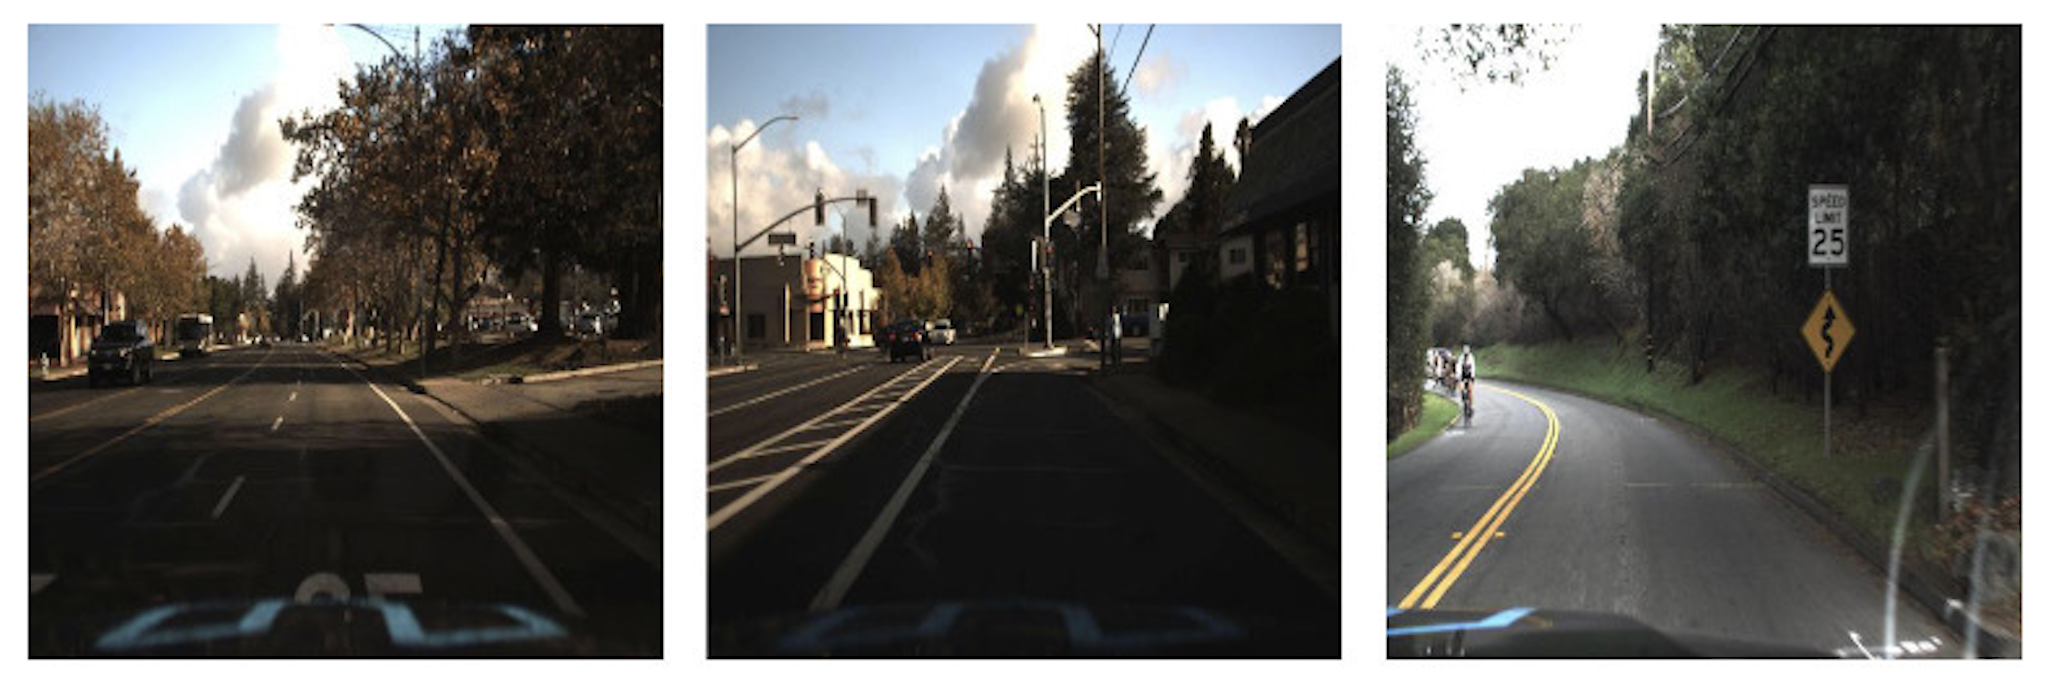
\includegraphics[width=0.55\linewidth]{datasetImages.png}
	\caption[Beispielbilder aus dem Datensatz]{Beispielbilder aus dem Datensatz. Quelle: \cite{datasetSelfDrivingCar}}
	\label{fig:datasetImages}
\end{figure}

Die Bilder in dem Datensatz umfassen verschiedene Szenarien im Straßenverkehr. Darunter befinden sich Stadt- und Landstraßen. Die Bilder wurden bei unterschiedlichen Lichtbedingungen aufgenommen, um ein breite Vielfalt an Situationen in den Daten abzudecken. 


\section{Klassenaufteilung}
Die ursprüngliche Klasseneinteilung ist in Abbildung \ref{fig:classDistributionRaw} dargestellt. Dort lässt sich erkennen, dass insbesondere die Aufteilung der Klasse \textit{Ampel} in Unterkategorien unterrepräsentiert ist. Um dieses Problem zu umgehen, wurden die \textit{Ampel}-Klassen zu einer Klasse \textit{trafficLight} zusammengeführt. Für das Auswerten des Datensatzes wurde dieser mit dem passenden Skript (datasetPreprocessing.ipynb) in einen Trainings-, Validierungs- und Testdatensatz aufgeteilt. Diese Aufteilung kann aus den farblichen Säulen in Abbildung \ref{fig:datasetTrainValTestSplit} entnommen werden. Eine weitere Bearbeitung des Datensatzes wurde nicht vorgenommen, um zu überprüfen, wie die verwendeten Netzwerke mit einem unbalancierten Datensatz umgehen. 

\begin{figure}
	\begin{subfigure}{0.5\textwidth}
		\centering
		\begin{tabular}{l|c|c}
			\hline
			Klassen & Anzahl & Index \\
			\hline
			\hline
			car & 64399 & 0 \\
			pedestrian & 10806 & 1 \\
			trafficLight-Red & 6870 & 2 \\
			trafficLight-Green & 5465 & 3 \\
			truck & 3623 & 4 \\
			trafficLight & 2568 & 5 \\
			biker & 1846 & 6 \\
			trafficLight-RedLeft & 1751 & 7 \\
			trafficLight-GreenLeft & 310 & 8 \\
			trafficLight-Yellow & 272 & 9 \\
			trafficLight-YellowLeft & 14 & 10 \\
			\hline
		\end{tabular}
		\caption{Klassenverteilung der rohen Daten als Tabelle}
		\label{tab:classDistributionRaw_graph}
	\end{subfigure}%
	\begin{subfigure}{0.5\textwidth}
	\centering
	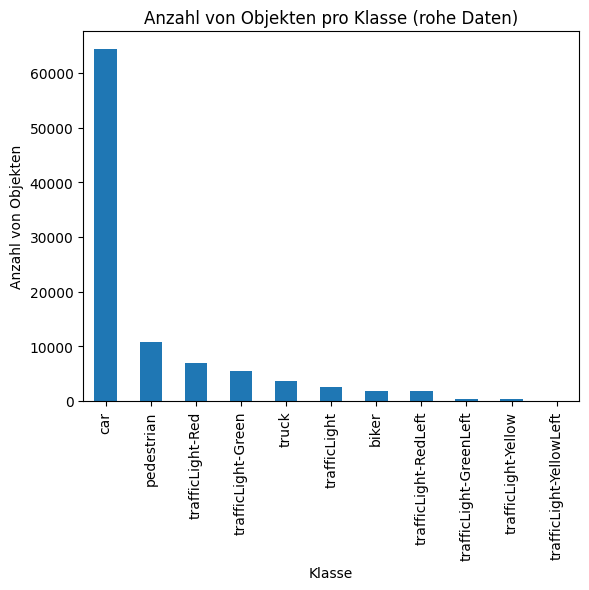
\includegraphics[width=\linewidth]{classDistribution_raw.png}
	\caption[Klassenverteilung der rohen Daten als Diagramm]{Klassenverteilung der rohen Daten als Diagramm. Quelle: Eigene Aufnahme}
	\label{fig:classDistributionRaw_graph}
	\end{subfigure}%
	\caption{Klassenverteilung der rohen Daten}
	\label{fig:classDistributionRaw}
\end{figure}


\begin{figure}
	\centering
		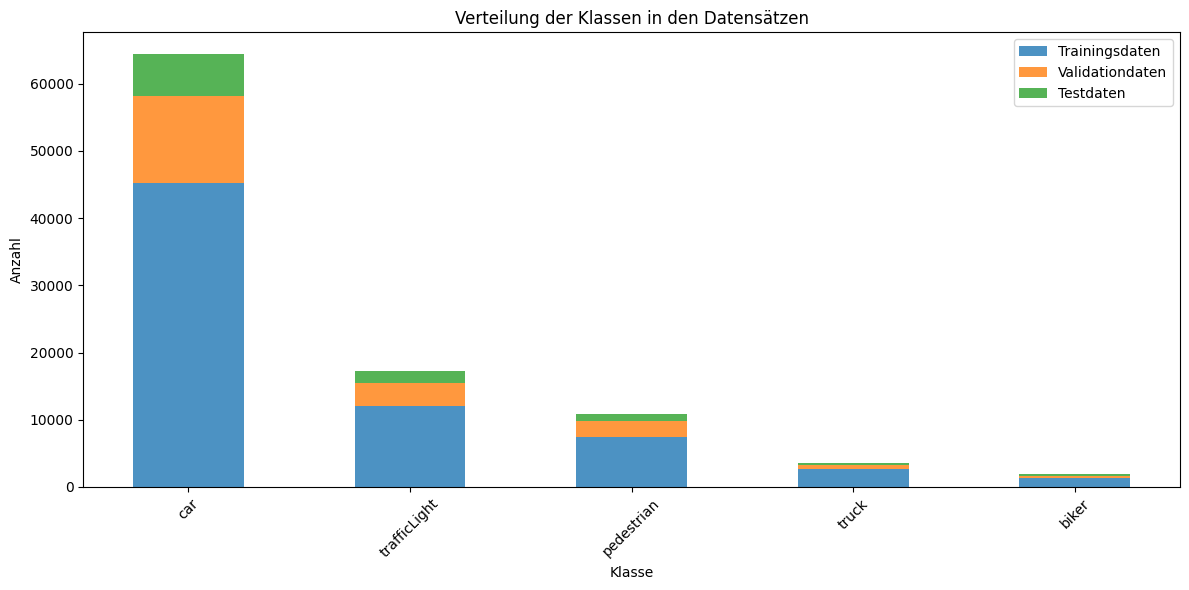
\includegraphics[width=\linewidth]{classDistribution_newClassesTrainValTest.png}
		\caption[Aufteilung in Trainings-, Validation- und Testdaten]{Aufteilung in Trainings-, Validation- und Testdaten. Quelle: Eigene Aufnahme}
		\label{fig:datasetTrainValTestSplit}
\end{figure}


\section{Aufbau}
\subsection{Rohdaten}
Die Rohdaten sind in einem Ordner gespeichert. Dieser Ordner enthält die Bilder im .jpg-Format und eine .csv-Datei in der alle Annotationen enthalten sind. Der Header der Datei enthält den Dateinamen des Bildes, die Breite und Höhe, die Klasse und die vier Bounding Box Koordinaten zu jedem Objekt.

Die folgenden Umwandlungen in die Formate werden mit dem Skript \textit{datasetConvertion.ipynb} gemacht. Die jeweiligen Ordnerstrukturen können in Kapitel \ref{chap:appendix} nachgelesen werden.


\subsection{YOLOX}
Das Netzwerk kann das COCO-Format und das PASCAL VOC-Format verarbeiten. In der folgenden Arbeit wird das COCO-Format verwendet. Zu diesem Zweck werden die Annotationen in einem separaten Ordner und die jeweiligen Bilddateien für Training, Validierung und Test ebenfalls in einem separaten Ordner abgelegt. Die Annotationen zu den drei Teildatensätzen liegen im .json-Format vor. Dabei wird jeder Klasse, jedem Bild und jeder Annotation eine ID zugewiesen, die die Zuordnung der Objekte zu den jeweiligen Bildern ermöglicht. 



\subsection{YOLOv8}
Dieses Netzwerk verwendet das YOLO-Format. Dabei werden die Bilder für Training, Validierung und Test in einem separaten Ordner gespeichert. Die dazugehörigen Labels stehen in einzelnen .txt-Dateien. Jedes Bild erhält eine zugehörige Textdatei mit dem gleichen Namen wie das Bild und der Struktur Klasse, x-Zentrum, y-Zentrum, Breite und Höhe. Die Koordinaten müssen auf die Bildgröße normiert sein. Die Labels liegen in einer korrespondierenden Ordnerstruktur. Die zugehörige Konfigurationsdatei gibt anschließend den Pfad zu den Datensatz und die Anzahl der Klassen an. 




  \chapter{Modell 1: YOLOX}\label{chap:yolox}
\section{Architektur}

\begin{figure}[h]
	\centering
	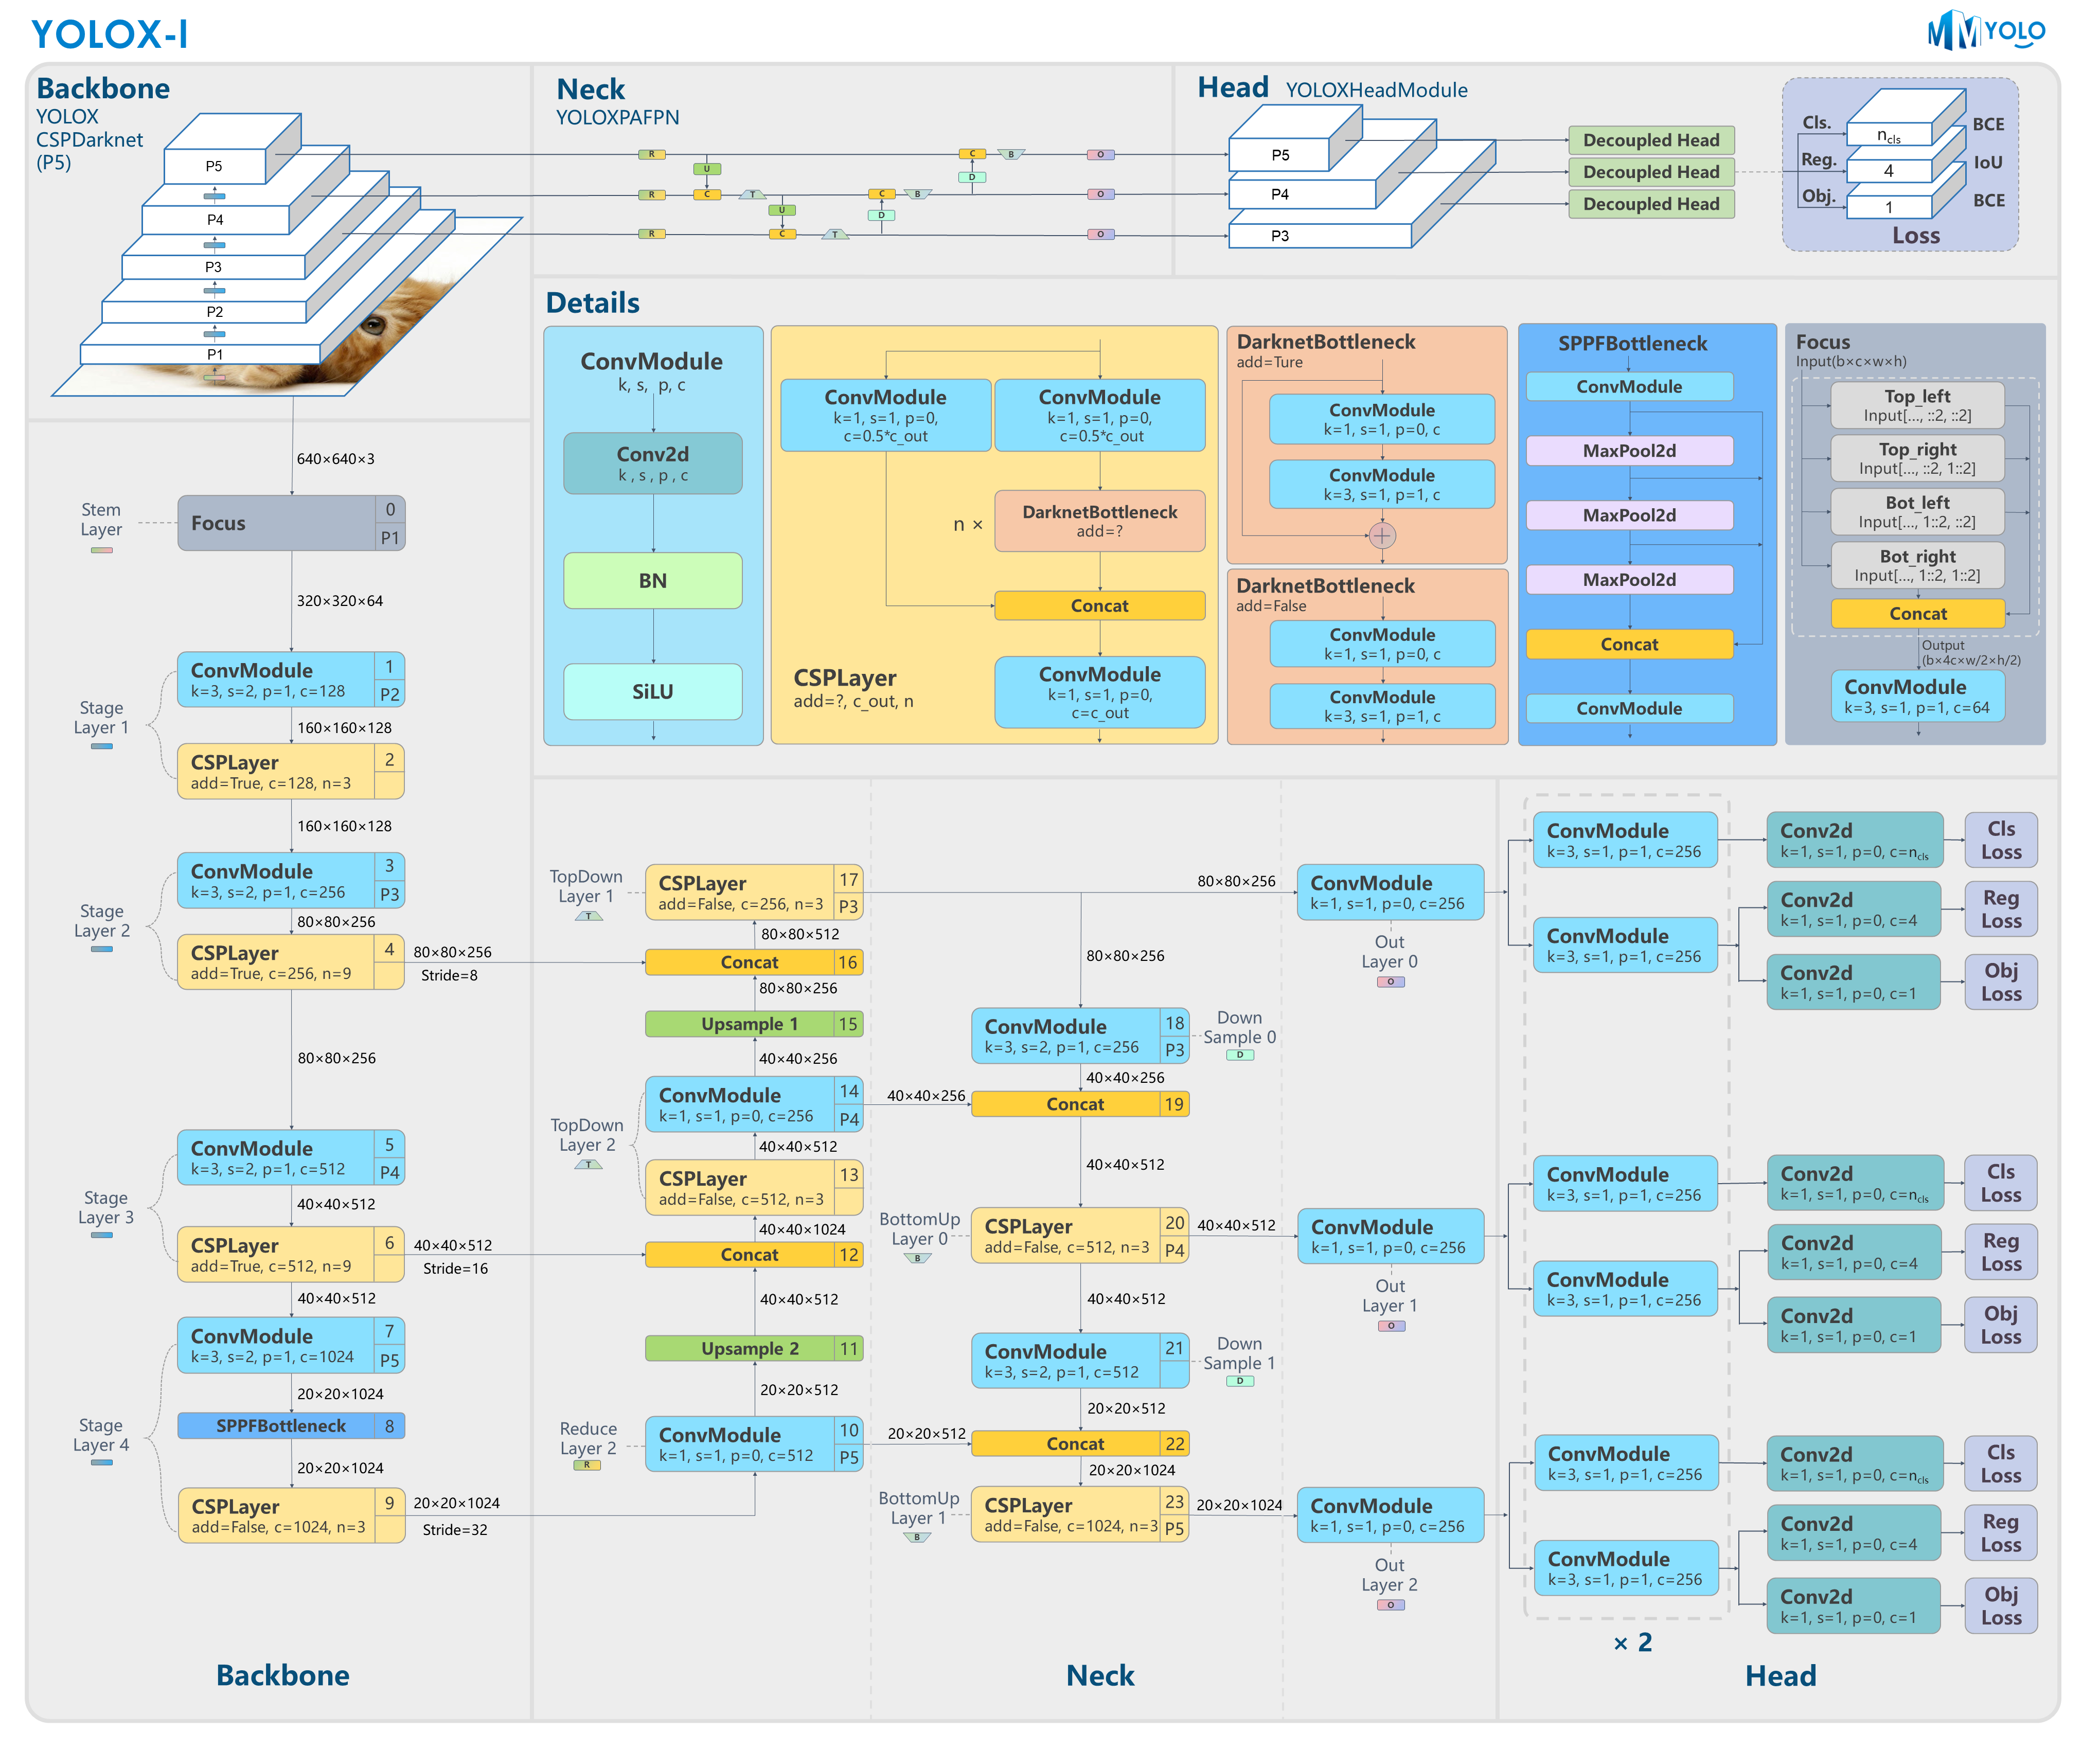
\includegraphics[width=0.8\linewidth]{yoloxArchitecture.png}
	\caption[Übersicht über die Architektur von YOLOX]{Übersicht über die Architektur von YOLOX. Quelle: \cite{yoloArchitecture, yoloxPaper, yoloxGitHubRepo}}
	\label{fig:yoloxArchitecture.png}
\end{figure}

Die YOLOX Architektur besteht aus einem Backbone-Netz, dem Neck und einem Head.

\subsection{Backbone}
YOLOX verwendet das CSPDarknet als Backbone, um Merkmale auf drei verschiedenen Maßstäben zu extrahieren. Die Ausgänge haben Dimensionen von ($H/8$x$W/8$x$256$), ($H/16$x$W/16$x$512$) und ($H/32$x$W/32$x$1024$). Diese Skalierungen ermöglichen die Erzeugung von Merkmalen für unterschiedliche Größen von Objekten. Durch die erhöhte Anzahl von Kanälen wird der Informationsverlust in den kleineren Feature-Maps ausgeglichen. Die tiefere Feature-Map (auf der Abbildung \ref{fig:yoloxArchitecture.png} unten) besitzt ein größeres Receptive Field und ein Pixel kodiert Informationen über einen größeren Bereich des ursprünglichen Bildes.

Das CSPDarknet (Cross Stage Partial) ist eine Modifizierung des ursprünglichen Darknet-Frameworks, das in YOLOv3 schon implementiert wurde. Die Anpassungen bieten Verbesserungen in Bezug auf Geschwindigkeit und Genauigkeit bei der Erkennung von Objekten in Bildern.

CSP steht für Cross Stage Partial Network. Diese Architektur besteht aus einem CSP-Block, der in verschiedenen Stufen des Netzwerks eingefügt ist. Der CSP-Block spaltet den Eingang in zwei Zweige auf, wobei ein Teil unverändert durch den Block läuft und der andere Teil durch eine Kombination aus Faltungsoperationen und Verbindungsschichten verarbeitet wird. Ziel der Kombination ist, dass das Netzwerk auf unterschiedlichen Ebenen des Netzwerks effektiver zu erfassen.

In dem Backbone wird außerdem noch am Ende der Verarbeitung ein SPP verwendet. SPP steht für Spartial Pyramid Pooling. Sie ermöglicht es Objekte unterschiedlicher Größen besser zu erkennen. Dass SPP-Modul teilt das Eingangsbild auf und reduziert die Dimensionen mithilfe von mehreren Pooling Operationen. Die unterschiedlichen Stufen werden anschließend wieder miteinander verbunden und weitergereicht. Ziel dieses Modul ist es Informationen von verschiedenen Skalierungen zu verbinden, um eine verbesserte Erkennung von Objekten zu gewährleisten. \cite{yoloxBackbone}

\subsection{Neck}
YOLOX verwendet im Neck das PAFPN (Path Aggregation Feature Pyramid Network). Dies ist eine Kombination des PAN (Path Aggregation Network) und dem FPN (Feature Pyramid Network). 

Das PAN ist verantwortlich für ds Zusammenführen von Informationen aus verschiedenen Netzwerkpfaden und die Integration dieser Informationen in einen einzigen Merkmalssatz. Es verbindet die Ausgänge des Backbone-Netzwerks auf unterschiedlichen Skalierungsebenen und passt die Dimensionen durch Upsampling aneinander an. Dadurch soll das Netzwerk ein umfassenderes Verständnis über die aus dem Backbone generierten Merkmale erhalten.

Das FPN ermöglicht eine robuste Objekterkennung in Bildern unterschiedlicher Skalierungen. Das Netzwerk erzeugt eine Hierarchie von Feature-Maps auf verschiedenen Skalierungen und verbindet sie miteinander. Dadurch sollen feine Details und auch semantische Informationen erfasst werden. FPN verwendet top-down und bottom-up-Verbindungen, um die Merkmale auf verschiedenen Ebenen des Netzwerks zu aggregieren. Die mit diesem Verfahren entstehende Merkmalspyramide wird an den Head weitergegeben. \cite{yoloxNeckPAN, yoloxNeckFPN}


\subsection{Head}
Der Head befindet sich am Ende des Netzwerks und ist für die Vorhersage der Objekte und deren Positionen in den Eingabebildern zuständig. Dort wird die Verlustfunktion berechnet. YOLOX verwendet einen Decoupled Head, der aus zwei Teilen besteht. Dieser Mechanismus ist mit YOLOX neu eingeführt worden und wird in Kapitel \ref{chap:decoupledHead} beschrieben.


\section{Methoden}
\subsection{Decoupled Head}\label{chap:decoupledHead}
Der Decoupled Head trennt die Vorhersage von Objekten und Bounding Boxes in zwei Zweige auf. Zusätzlich zum Pfad der Bounding-Box wird dort der Konfidenzwert vorhergesagt. Bei den herkömmlichen YOLO-Netzwerken wird die Vorhersage (Klasse, Bounding Box und Konfidenzwert) in einer einzigen Vorhersage gemacht. Dies kann zu Schwierigkeiten bei der Erkennung von Objekten unterschiedlicher Größe führen. 

Wie in der Abbildung \ref{fig:decoupledHead} (unten) zu sehen ist, wird im Decoupled Head die Dimension des Eingangs durch eine 1x1-Faltung reduziert und anschließend in zwei Pfade aufgeteilt. Das bedeutet, dass das Modell zuerst die Präsenz von Objekten vorhersagt und in einem parallelen Zweig die Bounding-Box-Koordinaten und den Objektscore für die erkannten Objekte berechnet. Dieser Head wird für jede der drei Neck-Feature-Maps ausgeführt. \cite{yoloxExplanationHowWorks}

Die drei Tensorausgaben von YOLOX enthalten die gleichen Informationen wie die Ausgänge des großen Tensors von YOLOv3:
\begin{itemize}
\item Cls: Die Klasse jeder Bounding Box
\item Reg: Die 4 Teile der Bounding Box
\item Obj: Wie sicher ist das Netzwerk, dass innerhalb der Bounding Box ein beliebiges Objekt ist
\end{itemize}


\begin{figure}[h]
	\centering
	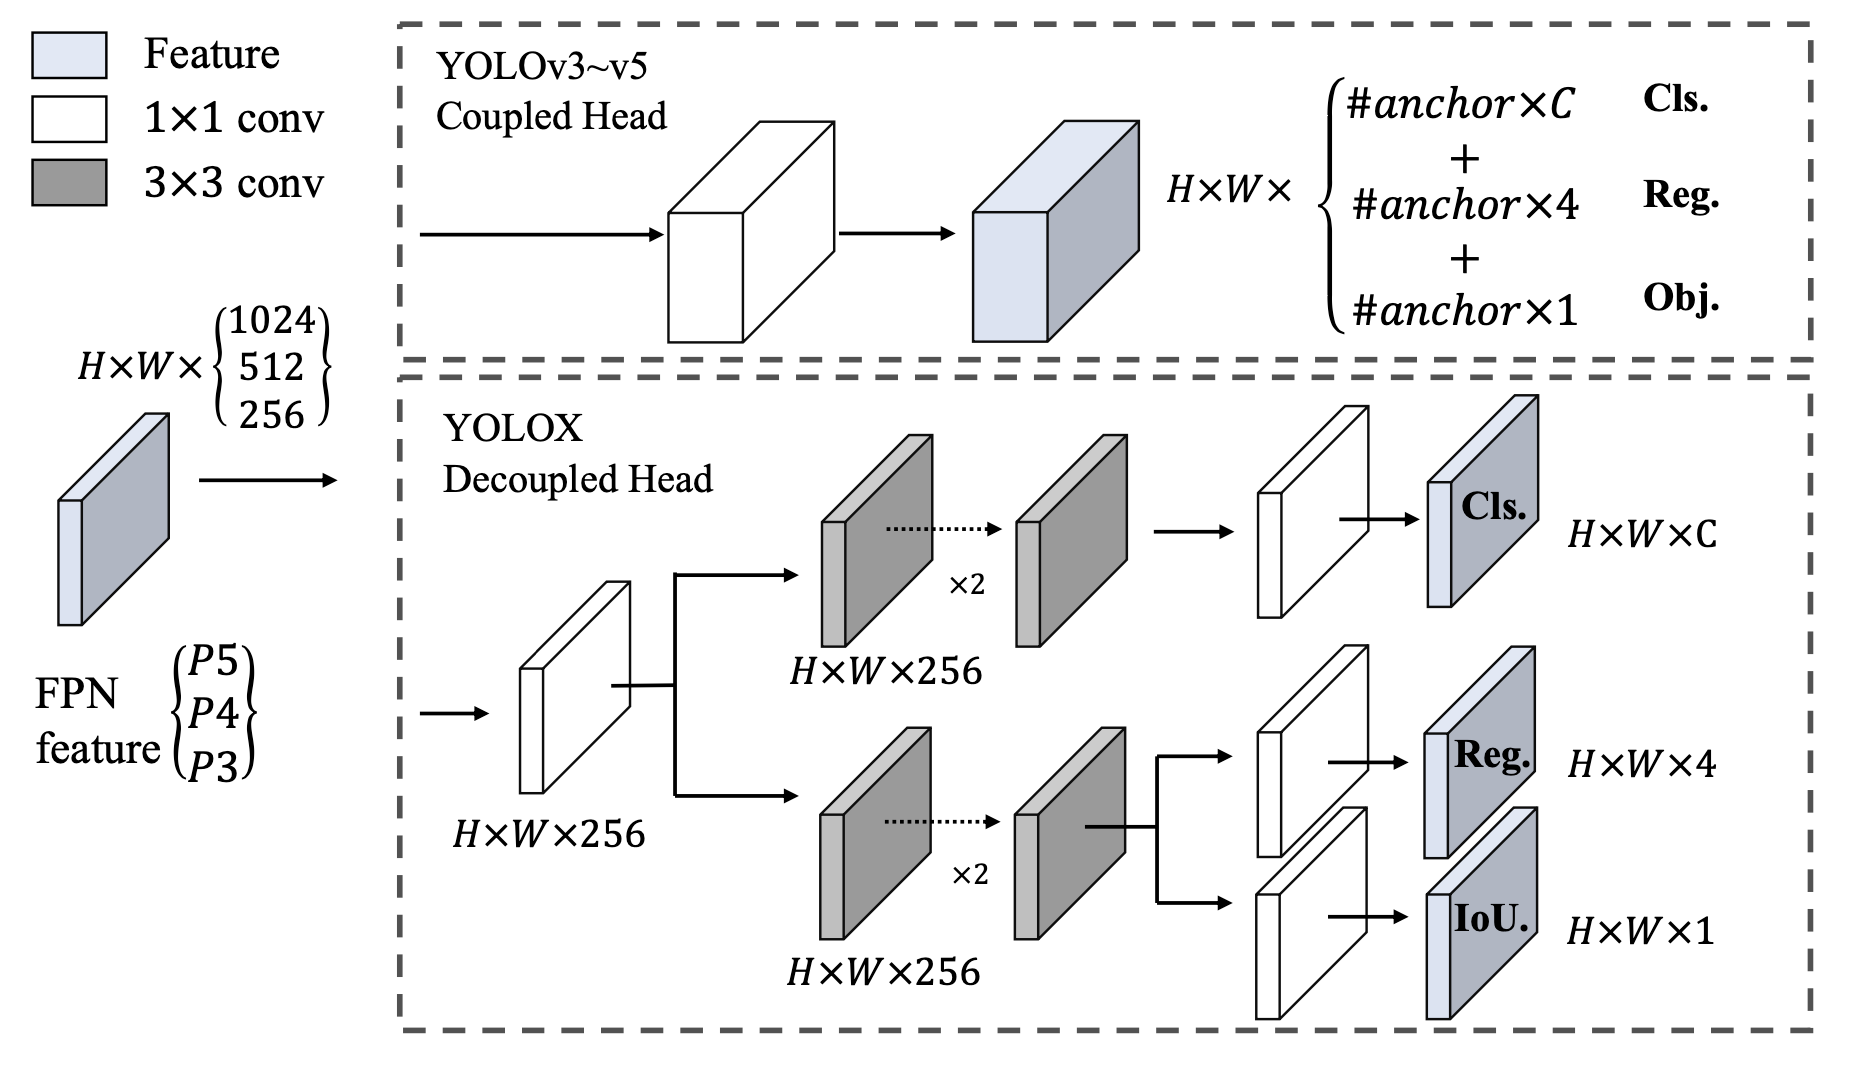
\includegraphics[width=0.55\linewidth]{decoupledHead.png}
	\caption[Illustration des Unterschieds zwischen dem Yolov3-Head und dem neuen Decoupled-Head ]{Illustration des Unterschieds zwischen dem YOLOv3-Head und dem neuen Decoupled-Head Quelle: \cite{yoloxPaper}}
	\label{fig:decoupledHead}
\end{figure}




\subsection{Anchor Free Prediction}\label{chap:anchorFree}
Bei der \textbf{Anchor-based Prediction} werden vordefinierte Ankerboxen verwendet, um Objekte in verschiedenen Größen zu repräsentieren. Diese Ankerboxen dienen als Referenzpunkte, auf die die Modelle während des Trainings ausgerichtet werden. Das Modell weißt der Ground-Truth (Echten) Box die ähnlichste Ankerbox zu und sagt die Verschiebung und Abmessungen der Ankerbox voraus, um sie dem Objekt anzupassen. Dazu muss vor Beginn des Trainings die Skalierung und Anzahl der Ankerboxen vorgegeben werden. Im Grunde ist eine Ankerbox eine Hilfe für das Modell, damit es nicht direkt eine Bounding Box vorhersagen muss.


Die implementierte Methode zur \textbf{Anchor-Free Predictio}n entstammt ursprünglich aus dem Paper ''FCOS: Fully Convolutional One-Stage Object Detection'' \cite{yoloxAnchorFree}. Anstelle von Ankerboxen verwendet die Anchor-Free-Methode ein Grid-basiertes Konzept. Im YOLOX Algorithmus wird eine Stride von 32, 16 und 8 verwendet, um die Ausgabebilder des Necks in ein Gitter zu unterteilen. Wenn ein Stride von 32 für ein 256×256 großes Bild verwendet wird, ergeben sich insgesamt 256/32 = 8 Schnittpunkte in jeder Dimension, also insgesamt 64 Schnittpunkte. Jeder dieser Schnittpunkte heißt Anker-Punkte. Ein Ankerpunkt ist ein Offset, mit dem die (x, y)-Position einer Vorhersage verschoben wird. Die Position des Ankers kann auf dem Bild mit den folgenden Formeln ermittelt werden:
\begin{align}
	x = \frac{s}{2} + s*i, \qquad y = \frac{s}{2} + s*j
\end{align}
Dabei ist s die Schrittweite, i ist der i-te Schnittpunkt auf der x-Achse und j ist der j-te Schnittpunkt auf der y-Achse. Bei YOLOX werden die Gitterpunkte als linker oberer Offset der Bounding Box verwendet. Die folgenden Formeln werden verwendet, um eine vorhergesagte Bounding Box $(p_x, p_y, p_w, p_h)$ auf die tatsächliche Position auf dem Bild $(l_x, l_y, l_w, l_h)$ abzubilden, wenn (x, y) der Schnittpunkt auf dem Gitter ist, zudem die Vorhersage gehört und s die Schrittweite der aktuellen FPN-Ebene ist:
\begin{align}
	l_x=p_x+x, \qquad l_y=p_y+y, \qquad l_w=s*e^{p_w}, \qquad l_h=s*e^{p_h}
\end{align}
Wir verschieben den vorhergesagten Punkt, indem wir die Vorhersage zum Anker-Punkt (dem (x,y)-Punkt, der dieser Vorhersage zugewiesen ist) hinzufügen. Durch die e-Funktion wird sichergestellt, dass die Höhe und Breite nicht negativ ist und verschieben diese auf der Grundlage der Schrittweite s eines Bildes. Das Beispiel zu dieser Methode kann in der angegeben Quelle nachgelesen werden. \cite{yoloxExplanationHowWorks}


\subsection{SimOTA Label Assignment}
Die Methode soll die Zuordnung der Vorhersagen zu den Ground-Truth-Objekten optimieren, da nicht alle Vorhersagen gut sind und das Modell nicht versuchen soll diese zu optimieren. Dazu werden die Anker-Punkte der vorherigen Methode von \ref{chap:anchorFree} in positive und negative Gruppen aufgeteilt. Die positive Gruppe beinhaltet ein Objekt und die negative Gruppe beinhaltet kein Objekt.

OTA (Optimal Transport Assignment) ist ein Ansatz, der das Zuordnungsproblem in der Objekterkennung als Optimal Transport (OT)-Problem formuliert. Es geht darum, den besten Plan zu finden, um Güter (Objekte) von Anbietern (Ground-Truth) zu Nachfragern (Vorhersagen oder Anker) zu minimalen Kosten zu transportieren. OTA verwendet OT, um die Labels den Ankerorten zuzuweisen und die Anker als positiv oder negativ zu kennzeichnen. Der Hintergrund wird als zusätzlicher "Lieferant" betrachtet. 

Das Problem des OTA-Algorithmus ist, dass dieser das Training verlangsamt. Aus diesem Grund gibt es eine Vereinfachung des Algorithmus, indem der optimale Zuweisungsplan angenähert wird. Vereinfacht funktioniert der Algorithmus folgendermaßen:
\begin{itemize}
	\item Berechne die Klassen- und Regressionsvorhersage für eine gegebene Eingabe durch das Modell.
	\item Erstelle einen Liefervektor, der das Angebot (durch Dynamic k estimation festgelegt) für jeden der Ground-Truths repräsentiert.
	\item Initialisiere den Nachfragevektor mit Einsen für jede Vorhersage.
	\item Berechne die Kosten für Klassenverluste ($FocalLoss(P^{cls}, G^{cls})$), Regressionsverluste ($IoULoss(P^{cls}, G^{cls})$))) und Zentrumsprior zwischen Vorhersagen und Ground-Truths.
	\item Berechne die Kosten für den Hintergrund und den Vordergrund basierend auf den Kosten der einzelnen Komponenten.
	\item Konstruiere eine Kostenmatrix, die die Hintergrund- und Vordergrundkosten enthält.
	\item Wähle die besten Vorhersagen basierend auf den Kosten und dem verfügbaren Angebot.
	\item Gebe die ausgewählten Vorhersagen zurück.
\end{itemize}

Der SimOTA-Algorithmus verwendet das Konzept von Angebot und Nachfrage, um die optimale Zuordnung zwischen Vorhersagen und Ground-Truths zu finden. Durch die Berücksichtigung von Kosten und verfügbarem Angebot werden die besten Vorhersagen ausgewählt, um eine präzisere Objekterkennung zu ermöglichen. Der vollständige Algorithmus kann in der angegeben Quelle nachgelesen werden.  \cite{yoloxExplanationSimOTA}


\subsection{Advanced Augmentation}
YOLOX verwendet Advanced Data Augmentation-Techniken wie Mosaic und MixUp, um die Datenvielfalt während des Trainings zu erhöhen und die Leistungsfähigkeit des Modells zu verbessern.

Beim \textbf{Mosaic}-Verfahrenwerden vier zufällig ausgewählte Bilder aus dem Trainingsdatensatz genommen und zu einem Mosaikbild kombiniert. Dabei werden die Bilder in vier quadratische Bereiche aufgeteilt und zu einem einzigen großen Bild zusammengefügt. Die Bounding Boxes der Objekte werden entsprechend angepasst und die Klassenlabels beibehalten. Mithilfe des CutOuts wird ein beliebiger Teil aus dem Bild ausgeschnitten und die Bounding Boxen noch einmal angepasst. Das Mosaikbild wird dann als Eingabe für das Modell verwendet. Der Grund für die Anwendung von Mosaic liegt darin, dass es die Fähigkeit des Modells verbessert, mit komplexen Szenarien und Überlappungen von Objekten umzugehen

\textbf{MixUp} ist eine Technik, bei der zwei zufällig ausgewählte Bilder und ihre entsprechenden Bounding Boxes und Klassenlabel gemischt werden, indem ihre Annotationen gewichtet kombiniert werden. Das erste Bild wird mit $\lambda$ und das zweite Bild mit $1-\lambda$ multipliziert. Die beiden resultierenden Ergebnisse werden addiert. \cite{yoloxExplanationAug}

\begin{figure}[h]
	\centering
	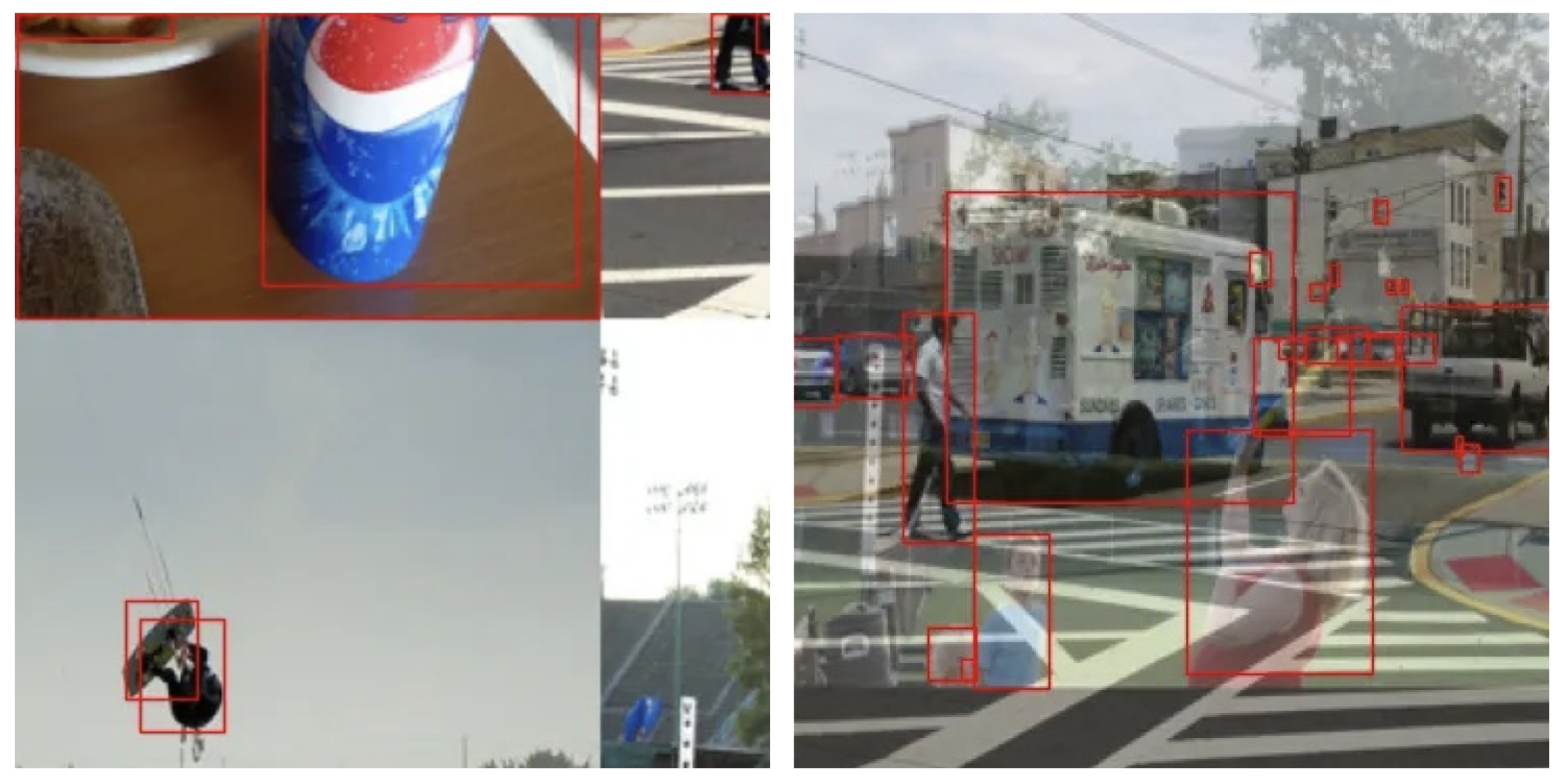
\includegraphics[width=0.55\linewidth]{dataAugmentation.png}
	\caption[Beispielbild nach Anwendung der beiden Data Augmentation Methoden]{Beispielbild nach Anwendung der beiden Data Augmentation Methoden (links: Mosaic, rechts: MixUp) Quelle: \cite{yoloxExplanationAug}}
	\label{fig:yoloxExplanationAug}
\end{figure}



\section{Verlustfunktion}
\subsection{Klassen}


\subsection{Bounding Box}


\subsection{Objectness}


\section{Modellauswertung}
  \chapter{Modell 1: YOLOv8}\label{chap:yolov8}
\section{Architektur}



\section{Verlustfunktion}



\section{Modellauswertung}
  \chapter{Zusammenfassung und Ausblick}\label{chap:conclusion}

  %\chapter{Vorlagen}

% Literaturverzeichnis \cite{label}
% Abbildungen, Tabellen, Listing, ... \autoref{label}


\section{Abbildungen}
% small h -> Latex legt fest wo Abbildung am besten liegt wegen Seitenaufteilung
% big H -> Abbildung genau an dieser stelle
\begin{figure}[h]
	\centering
	\includegraphics[width=0.55\linewidth]{sinus_plot.pdf}
	\caption[Beispiel Plot der Matplotlib Bibliothek]{Beispiel Plot der Matplotlib Bibliothek. Quelle: Eigene Aufnahme}
	\label{fig:sinus_plot}
\end{figure}


\section{Tabelle}
% l: linksbündig, c: zentriert, r: rechtsbündig
\begin{table}[H]
	\centering
	\begin{tabular}{l|c|c|c|c|c|c}
		&	Saplte 1	&	Spalte 2	&	Spalte 3	&	Spalte 4	&	Spalte 5	&	Spalte 6\\
		\hline
		Zeile 1		&	1	&	1	&	1 	&	1 &	1	&	1\\
		\hline
		Zeile 2	&	1	&	1	&	1	&	1	&	1		&	1\\
		\hline
		Zeile 3	&  1	&	1	&	1	&	1	&	1	&	1\\
		\hline
		Zeile 4	&	1	&	1	&	1	&	1	&	1	&	1
	\end{tabular}
\end{table}

\section{Programmiercode}
\lstinputlisting[caption=Matplotlib Beispiel Code. Quelle: Eigener Programmcode, label=code_Matplotlib, captionpos=b, firstline=1, lastline=11]{code/Matplotlib_Example.py}

\section{Mathematik}
\subsection{Matrix}
\begin{align}
	M =
	\begin{pmatrix}
		1 &	1	& 1 & 1\\
		1 & 1 & 1 & 1\\
		1 & 1 & 1 & 1\\
		1 & 1 & 1 & 1
	\end{pmatrix}
\end{align}


\subsection{Formel}

\begin{align}
	\begin{split}
		R(\alpha, \beta, \gamma) &=  R_z(\alpha) \cdot R_y(\beta) \cdot R_x(\gamma)\\
		&=\begin{pmatrix}
			C_\alpha\cdot C_\beta & -S_\alpha \cdot C_\gamma + C_\alpha \cdot S_\beta \cdot S_\gamma  & S_\alpha \cdot S_\gamma + C_\alpha \cdot S_\beta \cdot C_\gamma  \\
			S_\alpha\cdot C_\beta & C_\alpha\cdot C_\gamma + S_\alpha\cdot S_\beta\cdot S_\gamma & -C_\alpha\cdot S_\gamma + S_\alpha \cdot S_\beta \cdot C_\gamma \\
			-S_\beta & C_\beta \cdot S_\gamma & C_\beta \cdot C_\gamma
		\end{pmatrix}.
	\end{split}
	\label{EulerToRot}
\end{align}

\begin{equation*}
	[\bar{u}]_x \coloneqq
	\begin{pmatrix}
		0 & -\bar{u}_3 & \bar{u}_2 \\
		\bar{u}_3 & 0 & -\bar{u}_1 \\
		-\bar{u}_2 & \bar{u}_1 & 0 \\
	\end{pmatrix}
\end{equation*}

\begin{align}
	\label{VecToRot1}
	R = I + \sin(\theta)\cdot [\bar{u}]_x + (1-\cos(\theta))\cdot [\bar{u}]_x^2
\end{align}

\section{Aufzählung}
\begin{itemize}
	\item Item 1
	\item Item 2
	\item Item 3
	\item Item 4
\end{itemize}




\section{Station X: Zaun}
\subsection{Animation}
%Skirpt, Animator, Zustände zugreifen

\section{Weiteres}
%Name überlegen für Kapitel
%Animation für Igel Mutter -> von Magdalena -> Blend Tree 



  
 
  % Literaturverzeichnis
  \phantomsection
  \addcontentsline{toc}{chapter}{Literaturverzeichnis}
  \bibliographystyle{natdin}
  \bibliography{literatur}
  \newpage
  
  % Abbildungsverzeichnis
  \phantomsection
  \addcontentsline{toc}{chapter}{Abbildungsverzeichnis}
  \listoffigures
  \newpage

  %Tabellenverzeichnis
  %\phantomsection
  %\addcontentsline{toc}{chapter}{Tabellenverzeichnis}
  %\listoftables
  %\newpage
  
  %Anhang
 %\chapter*{Anhang}

\end{document}    